\documentclass[conference,a4paper]{template/IEEEtran}
\IEEEoverridecommandlockouts

\usepackage{cite}
\usepackage{amsmath,amssymb,amsfonts}
\usepackage{array}
\usepackage{booktabs}
\usepackage{float}
\usepackage{graphicx}
\usepackage{placeins}
\usepackage{tabularx}
\usepackage{textcomp}
\usepackage{xcolor}
\usepackage{url}
\usepackage{fontspec}

\setmainfont{Times New Roman}

\graphicspath{{../adnu/figures/}{../adnu/word/rendered_figures/}}
\renewcommand\IEEEkeywordsname{Keywords}
\newcolumntype{Y}{>{\raggedright\arraybackslash}X}
\setlength{\parskip}{0pt}

\def\BibTeX{{\rm B\kern-.05em{\sc i\kern-.025em b}\kern-.08em
    T\kern-.1667em\lower.7ex\hbox{E}\kern-.125emX}}

\begin{document}

\title{TinyML Smart Plug for Complementary Protection Against Progressive Fire-Inducing Electrical Faults in Residential Circuits}

\author{\IEEEauthorblockN{Francis M. Pe\~{n}a, Jett M. Lumabi, Alex A. Alferez, Referendo D. Soriano, Ph.D.}
\IEEEauthorblockA{\textit{Department of Electronics and Computer Engineering}\\
\textit{Ateneo de Naga University}\\
Naga City, Philippines}}

\maketitle

\begin{abstract}
Miniature circuit breakers remain essential but mainly address major
overcurrent and short-circuit events, leaving progressive socket-level
fire-inducing conditions less directly observed. This paper presents a
TinyML Smart Plug for complementary socket-level protection against sustained
overload, degraded socket-contact heating, and load-limited series arc faults
in 230V residential circuits. The prototype integrated calibrated sensing,
ESP32-S3 control, relay-based load isolation, Firebase logging, and
Progressive Web App (PWA) monitoring and labeling. Local firmware handled
thermal estimation, threshold protection, load-context classification,
Random Forest series-arc inference, fault latching, and relay actuation.
Evaluation included sensor validation, controlled overload, socket-heating,
and induced series-arc tests. Revalidation produced mean absolute errors of
3.910V, 0.178A, and 1.02$^{\circ}$C. The highest-stress overload case
reached 17.30A mean current and disconnected after 61.3s. Degraded sockets
heated faster than normal sockets: at about 9A, relay trip occurred at 52min
for the corroded socket and 120min for the normal socket; at about 13A, the
corroded and normal sockets tripped at 5min and 46min, respectively. Across
200 balanced normal and arc trials, the embedded model and firmware
persistence logic achieved 97.50\% accuracy, 98.97\% precision, 96.00\%
recall, and 97.46\% F1-score. The results support controlled laboratory
feasibility for a smart plug that complements mandatory residential
electrical protection.
\end{abstract}

\begin{IEEEkeywords}
ESP32-S3, series arc detection, socket-contact heating, sustained overload,
Random Forest, load-type classifier, multi-domain sensing.
\end{IEEEkeywords}

\section{INTRODUCTION}

Electrical faults remain a persistent residential fire concern. Philippine
fire incident reporting identifies electrical issues as a leading cause of
fires, while broader home-fire statistics also associate electrical failure
or malfunction with structure fires, injuries, and property losses
\cite{gma-bfp,nfpa-electrical}. The problem is not limited to
catastrophic short circuits. It also includes progressive electrical hazards
that may remain energized while producing thermal or waveform abnormalities
before conventional circuit protection is forced to operate.

Conventional residential protection remains essential. Branch-circuit
breakers, leakage protection, surge protection, and certified wiring
practice address the fault classes for which they are designed. However,
ordinary overcurrent protection is coordinated mainly around conductor
thermal protection and high-current events; it does not directly detect
progressive contact heating at a socket, persistent sub-trip overload
behavior, or low-current series arc faults that occur below the breaker
immediate trip region \cite{schneider-inverse,bal-pvc,lee-afci}. At the
plug-socket interface, a poor or degraded connection can generate localized
heating under otherwise ordinary current flow. A load-limited series arc can
also disturb the current waveform without producing a large RMS-current
increase.

This study distinguishes three progressive fire-inducing fault conditions.
Sustained overload is a current-persistence and time-stress problem.
Degraded socket-contact heating is a localized thermal problem in which the
hottest contact region may be hidden from an external thermistor. Series
arc faults are stochastic and load-dependent because normal nonlinear loads
can produce waveform behavior that may resemble arc-like disturbances. For
this reason, the prototype does not treat all abnormal conditions as one
generic fault state. Each condition requires protection basis that matches
its physical behavior.

The objective of this work was to design, develop, and evaluate an
ESP32-S3-based TinyML Smart Plug that provides complementary socket-level
protection for selected progressive fire-inducing electrical faults in
230V residential circuits. The work integrated calibrated voltage, current,
and temperature sensing; threshold-based overload and socket-heating
protection; load-context classification; Random Forest series arc-fault
inference; relay-based load isolation; fault latching; local audio-visual
alerts; Firebase logging; and Progressive Web App (PWA) monitoring, event
review, and data labeling.

The prototype uses a hybrid protection approach because the three target
fault conditions do not produce the same protection basis. Sustained
overload is handled through RMS-current level and persistence; degraded
socket-contact heating is handled through device temperature measurement
and compensated estimated socket temperature; and series arc-fault detection
is handled through load context, waveform features, Random Forest inference,
and firmware persistence logic. The evaluation was conducted under controlled
laboratory conditions involving overload, induced series arc fault, and
socket/contact-heating scenarios. The device is treated as a complementary
protective layer that operates alongside, not in place of, circuit breakers,
AFCIs, GFCIs, wiring inspection, and code-compliant residential protection.

\section{DESIGN BASIS AND SYSTEM OVERVIEW}

\subsection{Target Fault Classes}

The system was designed around progressive socket-level hazards. Overload
was treated as a sustained load-current condition. A warning may be
useful when the current is high, but immediate relay operation for every
short transient or inrush event would conflict with time-current
protection behavior. Thus, overload requires current persistence.

Degraded socket-contact heating was treated separately because poor
contact pressure, corrosion, looseness, or oxidation can increase local
contact resistance. Glowing-contact and receptacle-fire studies show that
this kind of poor connection can persist while the circuit still carries
load current \cite{meese-glowing,benfer-receptacle}. Recent poor-contact
fire studies likewise show the role of contact pressure, localized
heating, pyrolysis, and ignition progression \cite{zhang-poor-contact,li-ignition}.
Consequently, a local thermal estimate is needed even when current alone
cannot resolve the socket-contact condition.

Series arc faults were treated as a waveform-inference problem. A series
arc is load-limited, so it may not create a breaker-level current rise.
Instead, it can produce low-current gaps, current fluctuation, zero-region
behavior, harmonic disturbance, and high-frequency content
\cite{lee-afci,tian-arc-ai,zhao-zero,reji-thd,kim-hf}. Because normal
loads can also be nonlinear, the arc decision benefits from load context
and family-specific waveform interpretation \cite{medico-loads,shareef-nilm}.

The design basis is summarized in Table~\ref{tab:evidence}.

\begin{table}[H]
\caption{Fault Types and Protection Basis}
\label{tab:evidence}
\centering
\footnotesize
\setlength{\tabcolsep}{3pt}
\begin{tabularx}{\columnwidth}{@{}p{0.21\columnwidth}YY@{}}
\toprule
\textbf{Fault Type} & \textbf{Observed Behavior} & \textbf{Protection Basis}\\
\midrule
Sustained overload & Thermal stress from persistent load current & RMS-current threshold plus approximately 60s persistence score\\
Socket heating & Localized poor-contact heating at plug-socket interface & Thermistor input plus compensated estimated socket temperature\\
Series arc & Load-limited intermittent conduction and waveform disturbance & Load context, waveform features, Random Forest arc inference, and persistence counter\\
\bottomrule
\end{tabularx}
\end{table}

Each protection path asks a different question: whether current is
persistently high, whether the socket interface is thermally abnormal, or
whether the current waveform is repeatedly consistent with arcing under
the present load context.

\subsection{Hybrid Architecture}

Fig.~\ref{fig:architecture} shows the system architecture used in the
prototype. The sensing layer measures line voltage, load current, and
temperature near the plug/socket interface. The firmware layer performs
calibration, filtering, RMS calculations, temperature estimation,
waveform-feature extraction, load-context classification, TinyML arc
inference, protection-state evaluation, relay control, and event logging.
The cloud/PWA layer provides visualization, history review, labeling, and
operator interaction. The relay decision remains local to the firmware.

\begin{figure}[H]
  \centering
  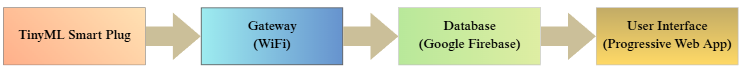
\includegraphics[width=\linewidth]{ch3/figure_3.2.png}
  \caption{System architecture of the TinyML Smart Plug.}
  \label{fig:architecture}
\end{figure}

The architecture is intentionally hybrid. Deterministic thresholds are
used where the protection evidence is direct and interpretable, as in
overload current and estimated socket temperature. TinyML is used where
the evidence is multi-feature, load-dependent, and ambiguous, as in
series arc-fault detection. The resulting protection process is local:
even if Wi-Fi or Firebase is unavailable, the ESP32-S3 can still evaluate
faults and engage relay isolation.

\section{METHODOLOGY}

\subsection{Hardware and Sensing Architecture}

Fig.~\ref{fig:hardware} shows the block diagram of the hardware implementation.
The prototype was built as a plug-through socket-level device for a
230V residential circuit. Its major elements were an ESP32-S3
microcontroller, ZMPT101B voltage-sensing channel, ACS37035 current
sensor, MCP3204 external 12-bit ADC, second-order anti-aliasing circuit,
10k$\Omega$ NTC thermistor, solid-state relay, relay latch, OLED display,
buzzer, low-voltage supply, and enclosed outlet assembly.

\begin{figure}[H]
  \centering
  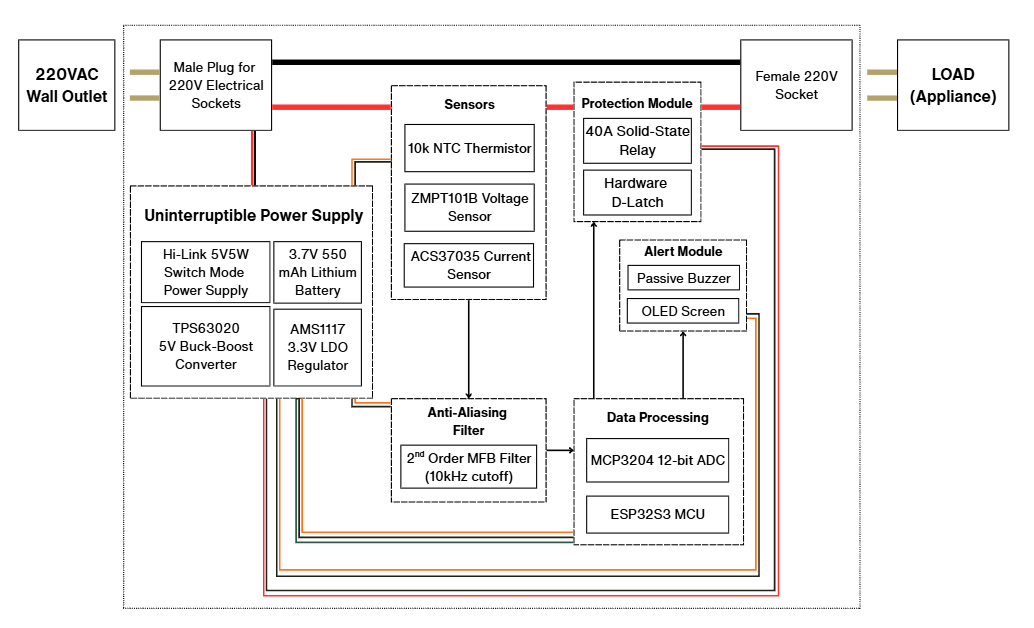
\includegraphics[width=\linewidth]{ch3/figure_3.4.png}
  \caption{Block diagram of the prototype hardware.}
  \label{fig:hardware}
\end{figure}

The current channel was central to the design. It supplied RMS current
for overload protection, a current-dependent term for socket-temperature
estimation, and waveform samples for feature extraction. The conditioned
current waveform was digitized through the MCP3204 and processed by the
ESP32-S3. The voltage channel supported RMS-voltage supervision and
mains-present interpretation. The thermistor was placed near the
plug-side wire-contact region and insulated to reduce direct ambient-air
influence. Because this point is necessarily offset from the hidden contact hotspot, the
thermal protection was based on compensated estimated socket temperature,
which represents the available external thermal measurement rather than a
direct internal-contact measurement.

The relay with a D-latch was the protective actuator. After a
confirmed trip condition, the relay disconnected the protected outlet and
the fault state remained latched until cleared. The OLED, buzzer, and PWA
provided alerts and user visibility. Firebase carried live telemetry,
history, CSV review, and operator fields, whereas the relay actuation path was
implemented in firmware and hardware.

\subsection{Firmware Protection Flow}

Fig.~\ref{fig:firmware-flow} summarizes the firmware protection flow
implemented in the prototype. On startup, the ESP32-S3 initializes the
sensors, ADC, relay driver, latch state, OLED, buzzer, Wi-Fi/Firebase
interface, and protection manager. The main loop then acquires slow
supervision variables and waveform frames in parallel: RMS voltage, RMS
current, thermistor temperature, and current-frame features.

\begin{figure}[H]
  \centering
  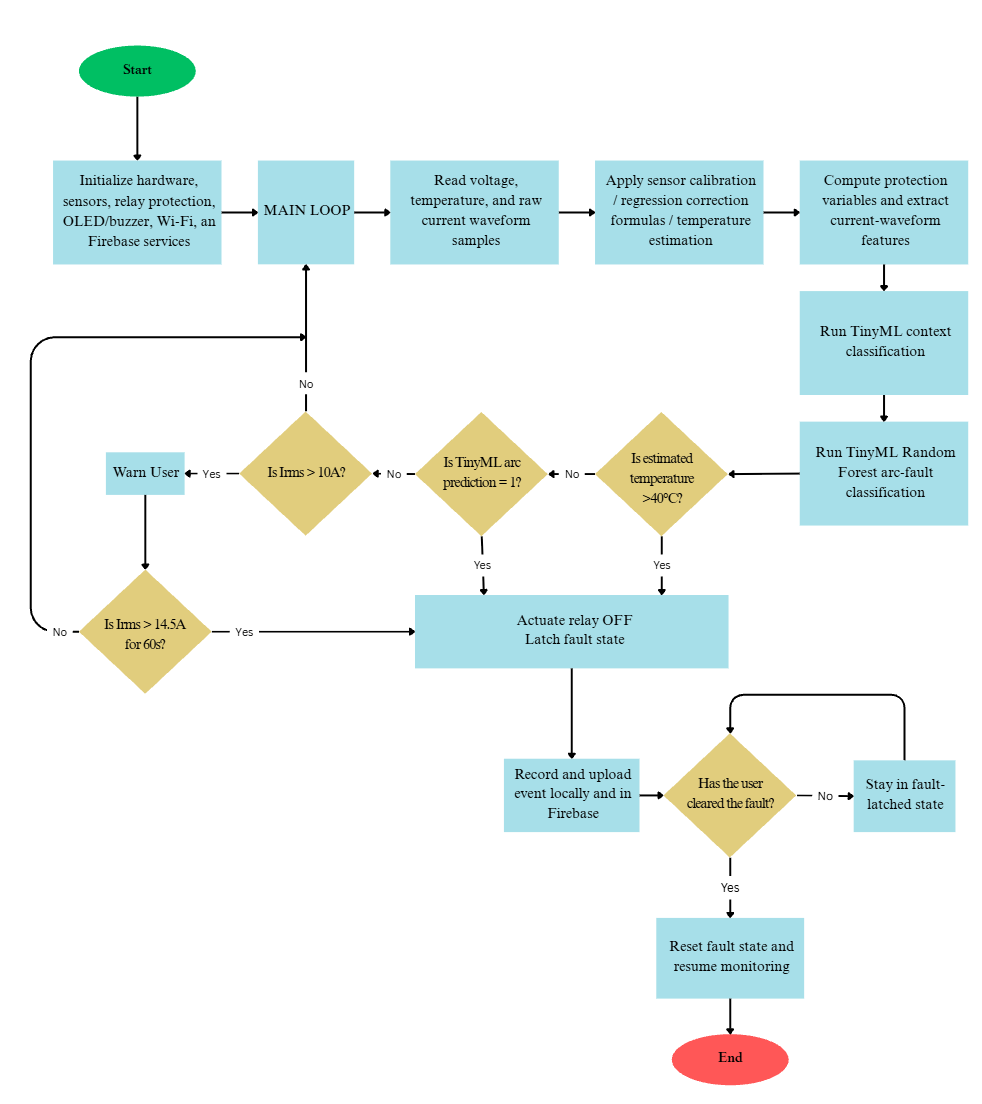
\includegraphics[width=\linewidth]{ch3/figure_3.3.png}
  \caption{Firmware flow for fault detection, relay actuation, and reset.}
  \label{fig:firmware-flow}
\end{figure}

The final relay decision occurs in the protection manager. Calibrated
voltage and current values feed deterministic voltage and overload
states. The temperature routine produces device temperature and estimated
socket temperature for thermal warning and trip evaluation. The waveform
path computes feature frames, updates load context, runs Random Forest
arc inference, and passes the arc output to a leaky persistence counter.
If overload, socket heating, or series arc evidence reaches its trip
condition, the firmware pulses the relay latch, records the fault, and
reports the fault state locally and through Firebase when available.
After relay isolation, the plug remains in a latched fault state until
the user clears the fault through local or PWA-supported interaction.

\begin{table}[t]
\caption{Firmware Protection Constants}
\label{tab:thresholds}
\centering
\footnotesize
\setlength{\tabcolsep}{3pt}
\begin{tabularx}{\columnwidth}{@{}p{0.25\columnwidth}p{0.30\columnwidth}Y@{}}
\toprule
\textbf{Function} & \textbf{Warning or model condition} & \textbf{Relay-trip condition}\\
\midrule
Voltage supervision & Outside 200-250V band & Instant 170/260V, or 7s delayed low/high voltage\\
Overload & $I_{\mathrm{rms}}>10.0$A warning & 1s average current $\geq$14.5A for about 60s\\
Socket heating & 39.0$^{\circ}$C estimated temperature & Estimated socket temperature $\geq$40.0$^{\circ}$C\\
Series arc fault & Context-aware Random Forest output & Arc counter reaches 8; +2 for arc frame, -6 for normal frame\\
\bottomrule
\end{tabularx}
\end{table}

Socket heating had highest reported-fault priority because temperature
is the most direct local fire-risk indicator. Arc fault was evaluated
next because a series arc may be hazardous without sustained overcurrent.
Overload remained a relay-trip condition after the persistence criterion
was satisfied. The protection constants are listed in Table~\ref{tab:thresholds}.

\subsection{Sensor Calibration and Validation}

Voltage and current calibration used polynomial correction because the
raw sensor outputs showed offset and scale nonlinearity across the tested
range. The voltage channel was calibrated
and revalidated against a Fluke 115 True RMS multimeter. The current
channel was calibrated using appliance load combinations and revalidated
against an Ingco clamp meter. The thermistor channel used the NTC
divider and Beta-equation conversion, then was compared against an
infrared thermometer at the external thermistor measurement point.

The validation procedure assessed protection-grade suitability rather
than traceable metrology. Voltage validation checked whether calibrated readings
were adequate for supply-state supervision. Current validation checked
whether RMS-current error was small relative to warning and trip
thresholds. Temperature validation checked the thermistor measurement at
its own location only. Hidden-contact temperature was treated separately
through degraded-contact experiments and conservative thermal estimation,
because standards and thermal-measurement literature caution that
external temperatures may lag or under-read internal contact points
\cite{iec-60884,vishay-ntc,watlow-placement,wilson-contact,dziarski-relay}.

\subsection{Overload Protection Method}

Overload testing used high-power load combinations connected through the
prototype. The firmware issued warning-level alerts above 10.0A while
retaining relay closure during warning-level excursions. A sustained trip
required the 1s current average to remain at or above 14.5A long
enough for the overload score to reach six. Since the score increments
every 10s, this corresponds to approximately 60s of persistent
overload. This design choice prevents
momentary current peaks and short transients from being treated as
confirmed overload trips while still responding to persistent current
stress.

The overload score can be represented by
\begin{equation}
S_{\mathrm{OL}}[k]=
\begin{cases}
\min(6,S_{\mathrm{OL}}[k-1]+1), & I_{\mathrm{avg}}\geq14.5\mathrm{A},\\
\max(0,S_{\mathrm{OL}}[k-1]-1), & I_{\mathrm{avg}}\leq14.1\mathrm{A}.
\end{cases}
\end{equation}
The relay trips when $S_{\mathrm{OL}}=6$. The method was evaluated by
recording mean voltage, mean current, peak current, warning state, relay
state, and trip latency during each load case.

\subsection{Socket-Heating Method}

Socket-heating evaluation used normal and intentionally degraded socket
contacts under matched load cases. The degraded-contact trials served as
accelerated laboratory comparisons rather than direct household field-fault
replicas, allowing controlled observation of contact-heating behavior. For
each trial, the prototype recorded device temperature from
the external thermistor, estimated socket temperature from firmware, and
relay state. An infrared thermometer supplied a reference terminal or
contact-region reading for interpretation.

The firmware thermal model separated three thermal quantities. First,
$T_{\mathrm{NTC}}$ was the direct external thermistor or device
temperature. Second, $T_{\mathrm{normal,exp}}$ was the expected normal
socket temperature for a healthy contact carrying the measured current
history. Third, $T_{\mathrm{socket,est}}$ was the relay-facing estimated
socket temperature used by the protection manager. This separation is
needed because the thermistor is outside the hidden contact hotspot. It
may lag or under-read the terminal region, while poor contact can generate
localized heating that RMS current alone cannot represent.

The estimator was implemented as a compact firmware model. The
current-shape term was computed as
\begin{equation}
s_I=\left[\mathrm{clamp}\left(\frac{I_{\mathrm{rms}}}{12.0},0,1.25\right)\right]^2,
\end{equation}
so the thermal term follows the current-squared tendency of resistive
heating while limiting extreme extrapolation. The expected normal term
used a slowly filtered healthy-contact rise, whose active-load target was
$\Delta T_{\mathrm{normal,target}}=0.20+12.0s_I$, added to the tracked
ambient or baseline temperature $T_a$:
\begin{equation}
T_{\mathrm{normal,exp}}=
\mathrm{clamp}(T_a+\Delta T_{\mathrm{normal}},-20,125).
\end{equation}
For an active load, the measured-temperature compensation was
\begin{equation}
\Delta T_{\mathrm{meas}}=0.30+1.20s_I,
\end{equation}
with the current-dependent rise forced toward zero when the load was
inactive. The protection-facing estimate was
\begin{equation}
\begin{aligned}
T_{\mathrm{comp}} &=
\mathrm{clamp}(T_{\mathrm{NTC}}+\Delta T_{\mathrm{meas}},-20,125),\\
T_{\mathrm{socket,est}} &=
\mathrm{clamp}\left(\max(T_{\mathrm{comp}},T_{\mathrm{normal,exp}}),
-20,125\right).
\end{aligned}
\end{equation}
The $\max(\cdot)$ operation prevents the relay-facing estimate from
falling below the expected normal socket heating for the same load while
still allowing measured local heating to dominate. The trip rule was
applied to $T_{\mathrm{socket,est}}$ so that raw thermistor readings and
current-dependent normal heating both influenced the thermal state. The
estimate should be interpreted as a conservative relay-facing variable,
with its behavior checked against normal and corroded-socket experiments
under comparable loads.

\subsection{TinyML and Arc-Fault Method}

Series arc detection used a two-stage load-aware TinyML pipeline. The
method followed the firmware order: current-frame acquisition, waveform
feature extraction, load-context classification, arc inference, and
persistence-filtered relay evaluation. The firmware computed 512-sample
current frames at a 27kHz target sampling rate with a 256-sample hop. A
Hann-windowed frequency analysis and time-domain calculations generated
waveform features; the Hann window was used to reduce spectral leakage
in discrete Fourier analysis
\cite{harris-dft}. Logged features supported training, PWA review, and
manual labeling.

The resulting TinyML processing sequence is shown in Fig.~\ref{fig:tinyml}.

\begin{figure}[!htbp]
  \centering
  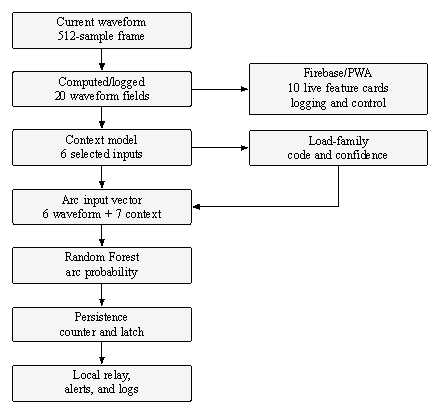
\includegraphics[width=0.90\linewidth]{fig_ch3_tinyml_sequence.pdf}
  \caption{TinyML processing flow for load-aware arc detection and relay actuation.}
  \label{fig:tinyml}
\end{figure}

In this sequence, a centroid-based context model classified load family
using six features: absolute RMS-current change, half-cycle asymmetry,
midband residual ratio, current THD, mid/high-frequency spectral flux,
and high-frequency energy delta. The firmware context schema defined six
possible family fields: resistive linear, inductive motor, rectifier
SMPS, phase-angle controlled, brush/universal motor, and other mixed.
The collected and tested signatures in this study were limited to
resistive loads, inductive loads, and brushed or universal-motor loads.
The context model standardized its six inputs, computed distance to the
stored load-family centroids, and accepted a family only when the best
confidence was at least 0.45. Otherwise, the arc model used its stricter
unknown-context threshold. This step was included because the same
waveform evidence has different meaning under different loads: harmonic
content and high-frequency variation may be normal for a brushed motor
but unusual for a resistive heater.

Only features used by the context model or by the deployed arc model are
listed in Tables~\ref{tab:context-features} and~\ref{tab:arc-features}.
The notation follows the firmware feature frame: $i_c[n]$ is the cleaned
current sample, $N=512$, $f_s$ is the sampling rate, $M_k$ is FFT magnitude,
$P_h$ is harmonic tone power, and $\epsilon$ is a small numerical offset.
Symbols beginning with $B$ denote adaptive healthy baselines maintained by
the firmware.

\begin{table}[!htbp]
\caption{Context-Model Feature Computations}
\label{tab:context-features}
\centering
\footnotesize
\setlength{\tabcolsep}{2.5pt}
\begin{tabularx}{\columnwidth}{@{}p{0.27\columnwidth}p{0.41\columnwidth}Y@{}}
\toprule
\textbf{Feature} & \textbf{Firmware computation} & \textbf{Context information}\\
\midrule
$\Delta I_{\mathrm{rms}}$ &
$|I_{\mathrm{rms}}[k]-I_{\mathrm{rms}}[k-1]|$ &
Load step and operating-state change\\
\addlinespace[1pt]
Half-cycle asymmetry &
$100|I_{\mathrm{pos}}-I_{\mathrm{neg}}|/[0.5(I_{\mathrm{pos}}+I_{\mathrm{neg}})]$ &
Positive/negative cycle imbalance\\
\addlinespace[1pt]
Current THD &
$100\sqrt{\sum_{h=2}^{10}P_h/P_1}$ &
Harmonic load signature\\
\addlinespace[1pt]
HF energy delta &
$10\log_{10}[(r_{\mathrm{HF}}+\epsilon)/(B_{\mathrm{HF}}+\epsilon)]$ &
High-frequency content relative to baseline\\
\addlinespace[1pt]
Midband residual ratio &
$20\log_{10}(R_{\mathrm{mid}}/B'_I)$ &
Non-harmonic residual structure\\
\addlinespace[1pt]
Mid/HF spectral flux &
$50\sum_{k=k_0}^{k_1}\left|\hat{M}_k-\hat{M}_{k,\mathrm{prev}}\right|$ &
Frame-to-frame spectral change\\
\bottomrule
\end{tabularx}
\end{table}

\begin{table}[!htbp]
\caption{Arc-Model Waveform Feature Computations}
\label{tab:arc-features}
\centering
\footnotesize
\setlength{\tabcolsep}{2.5pt}
\begin{tabularx}{\columnwidth}{@{}p{0.28\columnwidth}p{0.39\columnwidth}Y@{}}
\toprule
\textbf{Feature} & \textbf{Firmware computation} & \textbf{Arc evidence represented}\\
\midrule
Max low-current run &
$1000N_{\mathrm{run,max}}/f_s$ &
Longest extinction or weak-conduction gap\\
\addlinespace[1pt]
Zero-dwell ratio &
$100N_{\mathrm{near\ zero}}/N_{\mathrm{zc\ window}}$ &
Near-zero dwelling around crossings\\
\addlinespace[1pt]
Low-current ratio &
$100N^{-1}\sum\mathbf{1}(|i_c[n]|\leq I_{\mathrm{low}})$ &
Portion of weak-conduction samples\\
\addlinespace[1pt]
RMS-current z-score &
$|I_{\mathrm{rms}}-\mu_I|/(\sigma_I+\epsilon)$ &
Load-relative current departure\\
\addlinespace[1pt]
Midband residual ratio &
$20\log_{10}(R_{\mathrm{mid}}/B'_I)$ &
Non-harmonic residual energy\\
\addlinespace[1pt]
Mid/HF spectral flux &
$50\sum_{k=k_0}^{k_1}\left|\hat{M}_k-\hat{M}_{k,\mathrm{prev}}\right|$ &
Nonstationary spectral disturbance\\
\bottomrule
\end{tabularx}
\end{table}

In Tables~\ref{tab:context-features} and~\ref{tab:arc-features},
$\hat{M}_k=M_k/\sum_{r=k_0}^{k_1}M_r$ is the normalized magnitude spectrum
within the mid/high-frequency band, $r_{\mathrm{HF}}=E_{\mathrm{HF}}/
(E_{\mathrm{HF}}+E_{\mathrm{UM}})$, and
$R_{\mathrm{mid}}=\sqrt{E_{\mathrm{mid,res}}}/N$; $B'_I=\max(B_I,0.10)$
limits division by very small baselines. The low-current threshold is
$I_{\mathrm{low}}=\max(0.035,0.06\max(I_{\mathrm{rms}},0.10))$, which keeps
the conduction-gap tests load-relative while preserving a minimum near-zero
threshold.

The arc model was a Random Forest deployed as a C header in firmware.
Random Forest was selected because it can represent nonlinear feature
interactions while remaining exportable as a compact embedded ensemble
\cite{breiman-rf,pedregosa}. The deployed model used 13 inputs: six
waveform features and seven context fields. The waveform features were
maximum low-current run, zero-dwell ratio, low-current ratio, absolute
RMS-current z-score from baseline, midband residual ratio, and
mid/high-frequency spectral flux. The context fields were six one-hot
load-family inputs and one context-confidence input. The arc probability
threshold was 0.48 for supported confident contexts and 0.78 for unknown
context, with an additional minimum-feature-vote safeguard for unknown
loads. The selected Random Forest used 160 trees, a maximum depth of 16,
minimum leaf size of 4, minimum split size of 12, bootstrap sampling,
entropy splitting, and cost-complexity pruning alpha of 0.0001. The
deployed feature set can be summarized in four groups. First,
the conduction-gap inputs which are maximum low-current run, zero-dwell ratio,
and low-current ratio, represent extinction, weak conduction, and
near-zero dwell that can occur during separation and restrike. Second,
the current-departure input, expressed as an absolute RMS-current
z-score from the recent baseline, measures load-relative departure from
healthy operation. Third, the waveform-disturbance inputs, namely the
midband residual ratio and mid/high-frequency spectral flux, represent
residual spectral energy and frame-to-frame spectral change associated
with nonstationary arcing. Finally, the load-context inputs, composed of
six one-hot load-family fields and the context confidence, condition the
arc decision so that normal nonlinear loads are evaluated with
context-sensitive decision boundaries.

Training and testing were performed offline from firmware CSV logs.
Records were reviewed, manually labeled, cleaned with Python scripts,
split into training, validation, and reserved test views, and exported as
firmware headers. Fig.~\ref{fig:data-deploy} summarizes this workflow from
laboratory CSV records to embedded deployment. The final arc report used
35,512 training rows, 9,434 validation rows, and 10,268 reserved test rows.
Embedded testing then evaluated the exported model inside the firmware
protection path, where the model output was filtered by the arc persistence
counter before relay action. Thus, the reported trial result represents the
deployed protection pipeline, including embedded inference and counter-based
relay logic. This is different from reporting an offline classifier alone:
the relay result includes sensing, feature extraction, context gating,
model output, persistence scoring, and latch actuation.

\begin{figure}[H]
  \centering
  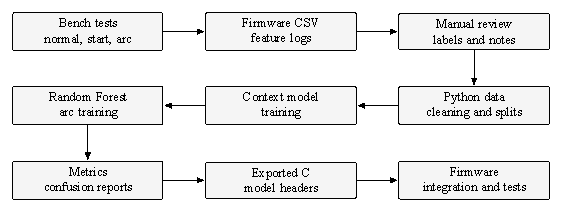
\includegraphics[width=\linewidth]{fig_ch3_data_labeling_deploy.pdf}
  \caption{Data labeling, model export, and embedded deployment workflow.}
  \label{fig:data-deploy}
\end{figure}

Table~\ref{tab:arc-data-prep} gives the corresponding dataset-preparation
counts. The small number of arc-label rows relative to normal-label rows
explains why the embedded detector was evaluated using precision, recall,
F1-score, and trial behavior rather than accuracy alone. It also explains
why firmware persistence was used: a single arc-like frame was not treated
as enough evidence for relay isolation.

\begin{table}[H]
\caption{Arc-Fault Dataset Preparation Summary}
\label{tab:arc-data-prep}
\centering
\footnotesize
\setlength{\tabcolsep}{3pt}
\begin{tabularx}{\columnwidth}{@{}Yr@{}}
\toprule
\textbf{Preparation item} & \textbf{Count}\\
\midrule
Raw CSV rows before cleaning & 55,085\\
Rows retained after cleaning & 49,296\\
Rows removed during cleaning & 5,789\\
Trainable rows & 45,010\\
Normal-label rows & 49,013\\
Arc-label rows & 283\\
Arc-training rows & 30,821\\
Load-context rows & 18,475\\
\bottomrule
\end{tabularx}
\end{table}

\FloatBarrier
\subsection{PWA, Firebase, and Logging Role}

The PWA and Firebase backend supported the research workflow by showing
live voltage, current, device temperature, estimated socket temperature,
context family, arc output, relay status, event history, and waveform
features. They also supported CSV inspection, data labeling, and operator
fault clearing. These functions improved observability and reproducibility
during laboratory trials. The local ESP32-S3 firmware remained responsible for protection-state
evaluation and relay isolation.

\FloatBarrier
\section{RESULTS AND DISCUSSION}

\subsection{Sensor Validation}

Table~\ref{tab:sensor-validation} summarizes the revalidation results.
Voltage MAE was 3.910V, current MAE was 0.178A, and temperature MAE was
1.02$^{\circ}$C. These errors were small relative to the implemented
thresholds. Current error, for example, was much smaller than the
separation between the 10.0A warning threshold and 14.5A sustained-trip
threshold. The temperature result validates the external thermistor
measurement point only; the socket-heating protection result is
interpreted through the compensated estimate and degraded-contact
tests.

\begin{table}[!htbp]
\caption{Sensor Validation Summary}
\label{tab:sensor-validation}
\centering
\small
\setlength{\tabcolsep}{4pt}
\begin{tabular*}{\columnwidth}{@{\extracolsep{\fill}}lccc@{}}
\toprule
\textbf{Channel} & \textbf{MAE} & \textbf{MSE} & \textbf{RMSE}\\
\midrule
Voltage & 3.910V & $15.539\mathrm{V}^2$ & 3.94V\\
Current & 0.178A & $0.04076\mathrm{A}^2$ & 0.202A\\
Temperature & 1.02$^{\circ}$C & $1.142^{\circ}\mathrm{C}^2$ & 1.07$^{\circ}$C\\
\bottomrule
\end{tabular*}
\end{table}

\subsection{Overload Protection}

Table~\ref{tab:overload} gives the overload evaluation. All heavy-load
trials exceeded the warning threshold, while relay operation occurred in
the highest-stress case. Trial 4 averaged 17.30A, reached a 19.73A peak,
and opened the relay after 61.3s. That trip time agrees with the intended
approximately 60s persistence behavior. Trials 1, 3, and 5 reached peaks
near or above the sustained threshold, then fell below the criterion
before accumulating the required persistence score. Thus, the overload
function behaved as time-aware complementary protection. Breaker
coordination and formal time-current compliance testing require a
separate standards-oriented evaluation.

\begin{table}[!htbp]
\caption{Overload Evaluation Results}
\label{tab:overload}
\centering
\small
\setlength{\tabcolsep}{3pt}
\begin{tabularx}{\columnwidth}{@{}cYccc@{}}
\toprule
\textbf{Trial} & \textbf{Load setup (WH: Water Heater)} & \textbf{\shortstack{Mean\\(A)}} & \textbf{\shortstack{Peak\\(A)}} & \textbf{\shortstack{Relay\\trip}}\\
\midrule
1 & 1.3kW kettle + WH & 12.87 & 14.85 & No\\
2 & 1.3kW kettle + 1.5kW kettle & 12.33 & 13.63 & No\\
3 & 1.5kW kettle + WH & 13.36 & 14.86 & No\\
4 & 1.3kW kettle + WH + 2 lamps & 17.30 & 19.73 & 61.3s\\
5 & 1.3kW kettle + WH + 1 lamp & 14.42 & 16.23 & No\\
\bottomrule
\end{tabularx}
\end{table}

\subsection{Socket-Heating Protection}

Socket-heating characterization showed that contact condition changed the
thermal outcome at similar current levels. The low-current protection
case is shown in Fig.~\ref{fig:heating-low}, while the severe
high-current case is shown in Fig.~\ref{fig:heating}. The paired figures
show the intended relay behavior across the tested range: lower-current
degraded-contact heating remained below the trip criterion, while the
severe case reached the relay-facing thermal threshold.

\begin{figure}[!htbp]
  \centering
  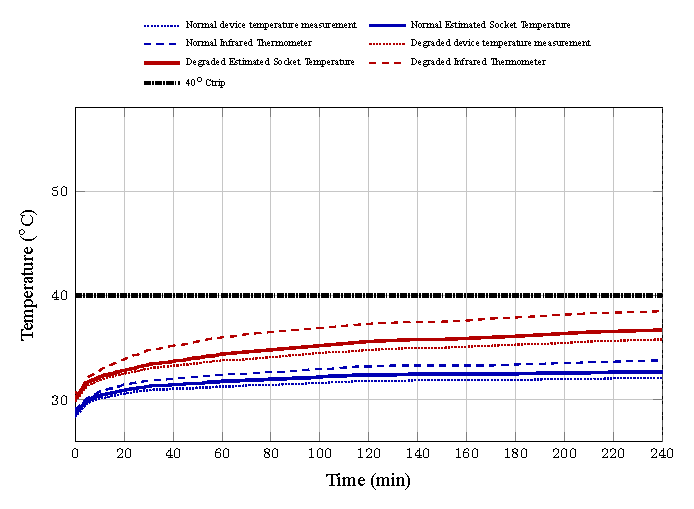
\includegraphics[width=\linewidth]{fig_ch4_protect_water_heater.pdf}
  \caption{Water-heater-only low-current socket-heating protection validation.}
  \label{fig:heating-low}
\end{figure}

\begin{figure}[!htbp]
  \centering
  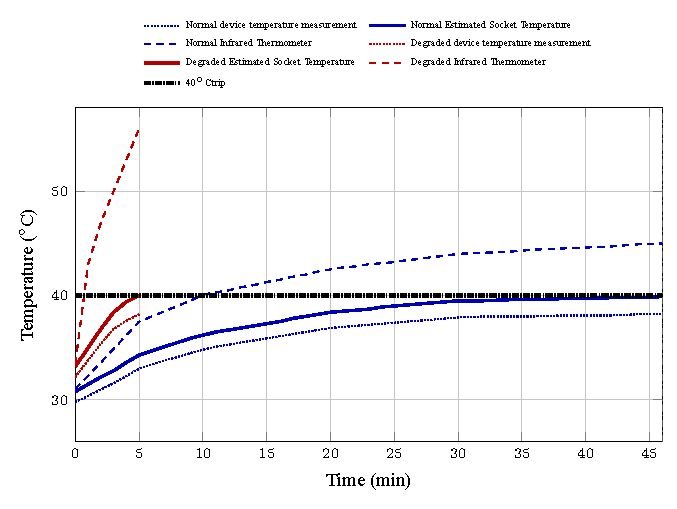
\includegraphics[width=\linewidth]{fig_ch4_protect_four_lamps.pdf}
  \caption{Water heater plus four halogen lamps during high-current socket-heating protection validation.}
  \label{fig:heating}
\end{figure}

Table~\ref{tab:heating} summarizes all socket-heating protection trials.
At about 5A in the water-heater-only case, neither socket tripped:
the corroded terminal ended hotter than the normal terminal
(38.5$^{\circ}$C versus 33.8$^{\circ}$C), but the estimated socket
temperature remained below the 40.0$^{\circ}$C relay criterion. At about
9A, the corroded socket reached the 38.2$^{\circ}$C comparison point in
48min, compared with 105min for the normal socket. At about 11A, the
corroded socket reached the same point in 7min, compared with 52min for
the normal socket. In the severe 13A corroded case, the relay tripped
after 5min and the reference terminal reached 56.0$^{\circ}$C. These
results support the premise that socket heating cannot be inferred from
RMS current alone. They also show that the thermal branch is a protection
function, not a corrosion classifier: at higher current levels, normal and
corroded sockets can both reach the conservative relay-facing threshold,
while the degraded socket shows faster rise and higher terminal
temperature under comparable loading.

The difference between device temperature, estimated socket temperature,
and IR terminal temperature is important. The prototype senses the
contact hotspot indirectly through an external thermistor and a
conservative relay-facing estimate. This approach provides socket-level
action before contact heating progresses further while preserving
non-trip behavior in low-current cases where the estimate remains below
threshold. The comparison therefore supports a complementary trip strategy
based on estimated thermal risk, while the IR terminal readings remain
interpretive references rather than the quantity directly measured by the
device.

\begin{table}[!htbp]
\caption{Socket-Heating Protection Summary}
\label{tab:heating}
\centering
\footnotesize
\setlength{\tabcolsep}{3pt}
\begin{tabularx}{\columnwidth}{@{}Ylccc@{}}
\toprule
\textbf{Load case (WH: Water Heater)} & \textbf{Socket} & \textbf{\shortstack{Mean\\(A)}} & \textbf{\shortstack{IR terminal\\($^{\circ}$C)}} & \textbf{Relay}\\
\midrule
WH & Normal & 5.17 & 33.8 & No\\
WH & Corroded & 4.85 & 38.5 & No\\
WH + 1 lamp & Normal & 7.11 & 40.3 & No\\
WH + 1 lamp & Corroded & 7.10 & 42.4 & Yes\\
WH + 2 lamps & Normal & 9.06 & 43.2 & Yes\\
WH + 2 lamps & Corroded & 9.04 & 44.1 & Yes\\
WH + 3 lamps & Normal & 11.07 & 43.9 & Yes\\
WH + 3 lamps & Corroded & 11.14 & 55.0 & Yes\\
WH + 4 lamps & Normal & 13.02 & 45.0 & Yes\\
WH + 4 lamps & Corroded & 13.08 & 56.0 & Yes\\
\bottomrule
\end{tabularx}
\end{table}

\subsection{Series Arc and TinyML Results}

The cleaned arc-training dataset contained 49,296 rows with 283 arc
markers, confirming that arc evidence was sparse and imbalanced in the
logged feature records, as shown earlier in Table~\ref{tab:arc-data-prep}. This imbalance supports the design choice of
interpreting relay-facing behavior at trial level, where embedded
inference, context gating, persistence counting, and relay actuation are
evaluated together.

The final relay-facing trial confusion matrix is shown in
Table~\ref{tab:arc-confusion}. Across 200 balanced normal and arc
trials, the deployed model and firmware persistence logic detected 96 of
100 arc trials and produced one false trip in 100 normal trials. The
corresponding performance metrics are shown in Table~\ref{tab:arc-metrics}.
Overall trial-level accuracy was 97.50\%, precision was 98.97\%, recall
was 96.00\%, and F1-score was 97.46\%. Trial-level metrics represent the
complete firmware behavior: repeated arc-like outputs accumulate toward a
relay decision, while isolated normal outputs decay.

\begin{table}[!htbp]
\caption{Series Arc-Fault Trial Confusion Matrix}
\label{tab:arc-confusion}
\centering
\small
\setlength{\tabcolsep}{4pt}
\begin{tabular*}{\columnwidth}{@{\extracolsep{\fill}}lcccc@{}}
\toprule
\textbf{Trial group} & \textbf{TP} & \textbf{FP} & \textbf{FN} & \textbf{TN}\\
\midrule
Recognized loads & 49 & 0 & 1 & 50\\
Unrecognized loads & 47 & 1 & 3 & 49\\
All tested loads & 96 & 1 & 4 & 99\\
\bottomrule
\end{tabular*}
\end{table}

\begin{table}[!htbp]
\caption{Series Arc-Fault Performance Metrics}
\label{tab:arc-metrics}
\centering
\small
\setlength{\tabcolsep}{3pt}
\begin{tabular*}{\columnwidth}{@{\extracolsep{\fill}}lcccc@{}}
\toprule
\textbf{Evaluation level} & \textbf{Accuracy} & \textbf{Precision} & \textbf{Recall} & \textbf{F1-score}\\
\midrule
Trial, recognized & 99.00\% & 100.00\% & 98.00\% & 98.99\%\\
Trial, unrecognized & 96.00\% & 97.92\% & 94.00\% & 95.92\%\\
Trial, all loads & 97.50\% & 98.97\% & 96.00\% & 97.46\%\\
\bottomrule
\end{tabular*}
\end{table}

\begin{table}[!htbp]
\caption{Load-Family Trial Results Summary}
\label{tab:arc-family}
\centering
\footnotesize
\setlength{\tabcolsep}{2.5pt}
\begin{tabularx}{\columnwidth}{@{}p{0.20\columnwidth}Ycc@{}}
\toprule
\textbf{Family} & \textbf{Tested loads} & \textbf{\shortstack{Arc\\detected}} & \textbf{\shortstack{Normal\\correct}}\\
\midrule
\shortstack[l]{Resistive} & Water heater, halogen lamp, electric kettle, heat gun & 40/40 & 40/40\\
\shortstack[l]{Inductive} & 40W stand fan & 10/10 & 10/10\\
\shortstack[l]{Brushed/\\universal} & Handheld vacuum, Electrolux vacuum, angle grinder, bench cutter, impact drill & 46/50 & 49/50\\
\bottomrule
\end{tabularx}
\end{table}

\begin{table}[!htbp]
\caption{Per-Load Trial-Level Arc Performance}
\label{tab:arc-per-load}
\centering
\footnotesize
\setlength{\tabcolsep}{2.2pt}
\begin{tabularx}{\columnwidth}{@{}Yp{0.18\columnwidth}rrrr@{}}
\toprule
\textbf{Load} & \textbf{Family} & \textbf{Acc.} & \textbf{Prec.} & \textbf{Rec.} & \textbf{F1}\\
\midrule
Water heater & Resistive & 100\% & 100\% & 100\% & 100\%\\
Halogen lamp & Resistive & 100\% & 100\% & 100\% & 100\%\\
Electric kettle & Resistive & 100\% & 100\% & 100\% & 100\%\\
40W stand fan & Inductive & 100\% & 100\% & 100\% & 100\%\\
Handheld vacuum & Brushed & 95\% & 100\% & 90\% & 94.74\%\\
Electrolux vacuum & Brushed & 95\% & 100\% & 90\% & 94.74\%\\
Angle grinder & Brushed & 95\% & 100\% & 90\% & 94.74\%\\
Bench cutter & Brushed & 95\% & 100\% & 90\% & 94.74\%\\
Impact drill & Brushed & 95\% & 90.91\% & 100\% & 95.24\%\\
Heat gun & Resistive & 100\% & 100\% & 100\% & 100\%\\
\bottomrule
\end{tabularx}
\end{table}

The selected arc features were physically consistent with the recorded
error pattern. Maximum low-current run, zero-dwell ratio, and
low-current ratio responded to conduction interruption rather than to
large RMS-current magnitude. The RMS-current z-score expressed departure
from the recent healthy baseline, so it remained load-relative. The
midband residual ratio and mid/high-frequency spectral flux captured
non-harmonic and nonstationary waveform disturbance after ordinary
periodic structure was reduced. These quantities gave clear trial
separation for the tested resistive and inductive loads, as shown in
Tables~\ref{tab:arc-family} and~\ref{tab:arc-per-load}.
The context features served a different role from the arc features.
$\Delta I_{\mathrm{rms}}$ and half-cycle asymmetry helped identify load
state and waveform shape; THD, high-frequency energy delta, residual
ratio, and spectral flux described the harmonic and nonstationary
signature of the operating load. Appending the resulting family and
confidence fields allowed the same arc-feature vector to be interpreted
with different thresholds for supported and unknown contexts.

The remaining trial-level errors were concentrated in brushed or
universal-motor loads. The impact drill contributed the single normal
false trip, while several brushed-load cases contributed missed arc
trials. This behavior is consistent with the feature interpretation:
healthy commutation, startup, and nonlinear current in brushed motors can
produce high harmonic content, spectral variation, and current
irregularity that partially overlap with arc indicators. The context
features in Table~\ref{tab:context-features} were therefore important
because they described the load family before applying the arc model;
however, the tested context coverage remained limited to resistive,
inductive, and brushed or universal-motor families. Broader household
electronic-load coverage is required before the detector can be treated
as generally representative of residential loads.

\subsection{Integrated Protection Assessment}

The integrated results show complementary behavior among the three
protection paths. Overload protection addressed persistent current stress
without tripping every transient. Socket-heating protection responded to
degraded-contact thermal behavior that current alone could not identify.
Series arc protection used waveform features and context to address a
load-limited fault that may remain below conventional overcurrent
operation. These results indicate the value of separating evidence by
fire-inducing mechanism while combining the outputs in one local
relay-protection pipeline.

The demonstrated behavior is bounded by the laboratory scope: selected
loads, induced faults, and bench conditions. Certification, field
readiness, and full residential nuisance-immunity evaluation require
separate future work.

\subsection{Scope and Limitations}

The study was conducted under controlled laboratory conditions. Long-term
deployment in occupied homes, aged installations, large appliance
populations, full branch-circuit diversity, and naturally occurring
faults were outside the evaluation scope. The load set and fault
conditions were limited by safe bench testing, especially for induced
series arcs.

The arc model may produce nuisance detections or missed detections on
unseen loads. Although the firmware context schema retained six possible
family fields, the collected and tested load signatures were limited to
resistive, inductive, and brushed or universal-motor loads. Sensitive
SMPS loads, phase-angle-controlled loads, and mixed electronic loads were
not included in comprehensive induced-fault coverage. The reported false positive
and false negative cases show that the dataset remains incomplete,
especially for brushed and nonlinear loads. The reported trial-level
metrics should therefore be read together with the confusion matrix and
load-family summary, not as a universal nuisance-immunity claim.

The thermal sensing method is indirect. The thermistor was located
outside the hidden contact spot, and the reference terminal reading often
exceeded the external device temperature and estimated socket
temperature. The 40.0$^{\circ}$C threshold is a prototype control
threshold for conservative relay action rather than a universal socket
safety limit or direct hotspot measurement.

Wi-Fi and Firebase supported monitoring, logging, labeling, and operator
interaction. Local relay protection was independent of cloud
connectivity, although remote visualization and history features were
reduced when the network was unavailable. The device provides supervision
at one socket rather than whole-house fault localization.

Certification-oriented testing was outside the present work. Creepage,
clearance, enclosure robustness, relay thermal rating, endurance,
electromagnetic compatibility, abnormal operation, and regulatory safety
tests remain future work. The implementation should be evaluated as
complementary socket-level supervision alongside breakers, AFCIs, GFCIs,
surge protection, code-compliant wiring, and professional electrical
assessment.

\section{CONCLUSION AND RECOMMENDATIONS}

The TinyML Smart Plug demonstrated controlled laboratory feasibility as a
hybrid socket-level protection implementation for selected progressive
fire-inducing electrical faults. As an ECE implementation, it integrates
calibrated sensing, deterministic protection logic, load-aware embedded
TinyML, relay latching, and monitoring support in one local protection
pipeline. The work also shows why the evidence must be
separated by mechanism: overload requires current persistence, degraded
socket-contact heating requires conservative thermal estimation, and
series arcs require load-aware waveform inference.

Within the tested scope, sensor errors were acceptable for the implemented
thresholds, the sustained overload function tripped the 17.30A case after
61.3s, degraded-contact tests showed faster and hotter socket behavior
than normal contacts, and the deployed arc pipeline achieved 97.50\%
trial-level accuracy while retaining the four missed arc trials and one
normal false trip in the analysis. These findings support feasibility for the proposed
complementary protection architecture.

Future work should expand the normal, nuisance, and arc-fault dataset
across more residential loads, plug conditions, contact gaps, and wiring
arrangements. Longer semi-field testing should support later
field-readiness evaluation. Thermal sensing should be improved through better
placement, multiple sensors, or stronger estimation models. Firmware and
hardware should be optimized for longer sampling, logging reliability,
and memory margin. Enclosure, insulation, relay rating, creepage,
clearance, strain relief, and thermal safety should be redesigned toward
certification-oriented testing. Arc labeling and trial annotation should
also be improved so future TinyML models can be trained with stronger
fault-transition evidence.

\section*{Acknowledgment}

The authors gratefully acknowledge their thesis advisor, Dr. Referendo D. Soriano, Ph.D., PECE,
for his technical guidance and supervision throughout the study. They also
thank Engr. Anacleto S. Casimiro, Dr. Joel R. Noche, and Engr. Jean Paul
I. Paje for their panel review, comments, and recommendations. The authors
extend their appreciation to Engr. Kris Lloyd Villamonte, Sir Jojo, Sir Bob,
and the laboratory personnel, electricians, families, and friends who
supported safe prototype construction and testing.

\begin{thebibliography}{00}
\IEEEtriggeratref{9}
\bibitem{gma-bfp} J. Rita and GMA Integrated News, ``Electrical issues remain most common cause of fire - BFP data,'' \textit{GMA News Online}, Feb. 28, 2025. [Online]. Available: \url{https://www.gmanetwork.com/news/topstories/nation/937689/electrical-issues-remain-most-common-cause-of-fire-bfp-data/story/}
\bibitem{nfpa-electrical} R. Campbell, ``Home fires caused by electrical failure or malfunction,'' NFPA Research Report. [Online]. Available: \url{https://www.nfpa.org/education-and-research/research/nfpa-research/fire-statistical-reports/home-fires-caused-by-electrical-failure-or-malfunction}
\bibitem{schneider-inverse} Schneider Electric, ``What is inverse time tripping? Are circuit breakers inverse time trip?'' [Online]. Available: \url{https://www.se.com/us/en/faqs/FA115818/}
\bibitem{bal-pvc} S. Bal and Z. A. Tamus, ``A method for assessing the degradation of PVC-insulated low-voltage distribution cables exposed to short-term cyclic aging,'' \textit{Electronics}, vol. 13, no. 6, Mar. 2024, doi: 10.3390/electronics13061085.
\bibitem{lee-afci} D. Lee, A. Trotta, and W. King Jr., ``New technology for preventing residential electrical fires: Arc-fault circuit interrupters (AFCIs),'' U.S. Consumer Product Safety Commission, 2003. [Online]. Available: \url{https://www.cpsc.gov/s3fs-public/AFCIFireTechnology.pdf}
\bibitem{meese-glowing} W. Meese and R. Beausoliel, ``Exploratory study of glowing electrical connections,'' NBSIR 76-1011, National Bureau of Standards. [Online]. Available: \url{https://nvlpubs.nist.gov/nistpubs/Legacy/IR/nbsir76-1011.pdf}
\bibitem{benfer-receptacle} M. Benfer and D. Gottuk, ``Development and analysis of electrical receptacle fires,'' U.S. Department of Justice, Sep. 2013. [Online]. Available: \url{https://www.ojp.gov/pdffiles1/nij/grants/243828.pdf}
\bibitem{zhang-poor-contact} J. Zhang, L. Huang, T. Chen, and G. Su, ``Simulation based analysis of electrical fire risks caused by poor electric contact between plug and receptacle,'' \textit{Fire Safety Journal}, vol. 126, p. 103434, Dec. 2021, doi: 10.1016/j.firesaf.2021.103434.
\bibitem{li-ignition} C. Li, Z. Yang, W. Yao, K. Zou, H. Liu, J. Lin, and S. Lu, ``Experimental study of ignition process caused by poor electrical contact of connector,'' \textit{Process Safety and Environmental Protection}, vol. 189, pp. 1517-1526, Sep. 2024, doi: 10.1016/j.psep.2024.07.006.
\bibitem{iec-60884} International Electrotechnical Commission, ``Plugs and socket-outlets for household and similar purposes - Part 1: General requirements,'' IEC 60884-1:2022, Aug. 2022. [Online]. Available: \url{https://cdn.standards.iteh.ai/samples/23612/a1e17dc388fe439b963c04ba4ca5c4c5/IEC-60884-1-2022.pdf}
\bibitem{vishay-ntc} Vishay, ``NTC thermistors,'' Resistive Products, Jan. 2021. [Online]. Available: \url{https://www.vishay.com/docs/29053/ntcappnote.pdf}
\bibitem{watlow-placement} Watlow, ``Determining sensor placement in a thermal system.'' [Online]. Available: \url{https://www.watlow.com/resources-and-support/engineering-tools/knowledge-base/sensor-placement-in-a-thermal-system}
\bibitem{wilson-contact} C. Wilson, G. McIntosh, and R. S. Timsit, ``Contact spot temperature and the temperature of external surfaces in an electrical connection,'' in \textit{26th International Conference on Electrical Contacts (ICEC 2012)}, IET, 2012, pp. 12-17, doi: 10.1049/cp.2012.0614.
\bibitem{dziarski-relay} K. Dziarski, L. Druzynski, A. Hulewicz, and J. Piechocki, ``Indirect thermographic measurement of the contact temperature of an electromechanical relay,'' \textit{Measurement Science Review}, vol. 26, no. 2, pp. 67-72, Mar. 2026, doi: 10.2478/msr-2026-0009.
\bibitem{saha-tinyml} S. S. Saha, S. S. Sandha, and M. Srivastava, ``Machine learning for microcontroller-class hardware: A review,'' \textit{IEEE Sensors Journal}, vol. 22, no. 22, pp. 21362-21390, Nov. 2022, doi: 10.1109/JSEN.2022.3210773.
\bibitem{tian-arc-ai} C. Tian \textit{et al.}, ``Arc fault detection using artificial intelligence: Challenges and benefits,'' \textit{Mathematical Biosciences and Engineering}, vol. 20, no. 7, pp. 12404-12432, 2022, doi: 10.3934/mbe.2023552.
\bibitem{zhao-zero} H. Zhao, J. Liu, and J. Lou, ``Series arc fault detection based on current fluctuation and zero-current features,'' \textit{Electric Power Systems Research}, vol. 202, p. 107626, Jan. 2022, doi: 10.1016/j.epsr.2021.107626.
\bibitem{reji-thd} G. Reji, K. Selvajyothi, and B. Raja, ``Investigating THD for series arc fault detection in single-phase electrical networks,'' in \textit{2024 6th International Conference on Energy, Power and Environment (ICEPE)}, IEEE, Jun. 2024, pp. 1-6, doi: 10.1109/ICEPE63236.2024.10668947.
\bibitem{kim-hf} Y.-S. Kim, D.-Y. Jang, and W.-C. Lee, ``Arc fault line detection in multi-load systems using high-frequency noise and zero-crossing period analysis,'' \textit{Journal of Electrical Engineering \& Technology}, vol. 21, no. 1, pp. 539-557, Aug. 2025, doi: 10.1007/s42835-025-02393-1.
\bibitem{medico-loads} R. Medico \textit{et al.}, ``A voltage and current measurement dataset for plug load appliance identification in households,'' \textit{Scientific Data}, vol. 7, no. 1, p. 49, Feb. 2020, doi: 10.1038/s41597-020-0389-7.
\bibitem{shareef-nilm} H. Shareef, M. Asna, R. Errouissi, and A. Prasanthi, ``Rule-based non-intrusive load monitoring using steady-state current waveform features,'' \textit{Sensors}, vol. 23, no. 15, Aug. 2023, doi: 10.3390/s23156926.
\bibitem{david-tflm} R. David \textit{et al.}, ``TensorFlow Lite Micro: Embedded machine learning on TinyML systems,'' arXiv:2010.08678, 2020. [Online]. Available: \url{https://arxiv.org/abs/2010.08678}
\bibitem{breiman-rf} L. Breiman, ``Random forests,'' \textit{Machine Learning}, vol. 45, no. 1, pp. 5-32, 2001, doi: 10.1023/A:1010933404324.
\bibitem{pedregosa} F. Pedregosa \textit{et al.}, ``Scikit-learn: Machine learning in Python,'' \textit{Journal of Machine Learning Research}, vol. 12, no. 85, pp. 2825-2830, 2011. [Online]. Available: \url{https://www.jmlr.org/papers/v12/pedregosa11a.html}
\bibitem{harris-dft} F. J. Harris, ``On the use of windows for harmonic analysis with the discrete Fourier transform,'' \textit{Proceedings of the IEEE}, vol. 66, no. 1, pp. 51-83, Jan. 1978, doi: 10.1109/PROC.1978.10837.
\end{thebibliography}

\end{document}
